%%%%%%%%%%%%%%%%%%%%%%%%%%%%%%%%%%%%%%%%%
% Short Sectioned Assignment
% LaTeX Template
% Version 1.0 (5/5/12)
%
% This template has been downloaded from:
% http://www.LaTeXTemplates.com
%
% Original author:
% Frits Wenneker (http://www.howtotex.com)
%
% License:
% CC BY-NC-SA 3.0 (http://creativecommons.org/licenses/by-nc-sa/3.0/)
%
%%%%%%%%%%%%%%%%%%%%%%%%%%%%%%%%%%%%%%%%%

%------------------------------------------------------------------------
%PACKAGES AND OTHER DOCUMENT CONFIGURATIONS
%------------------------------------------------------------------------

\documentclass[paper=a4, fontsize=11pt]{report} % A4 paper and 11pt font size
\usepackage[swedish, english]{babel}            % Swedish and English language/hyphenation
\usepackage[T1]{fontenc}                        % use 8-bit encoding that has 256 glyphs
\usepackage[a4paper]{geometry}
\usepackage{hyperref}
\usepackage[myheadings]{fullpage}
\usepackage{fancyhdr}
\usepackage{lastpage}
\usepackage{graphicx, wrapfig, subcaption, setspace, booktabs}
\usepackage[T1]{fontenc}
\usepackage[font=small, labelfont=bf]{caption}
\usepackage{fourier}
\usepackage[protrusion=true, expansion=true]{microtype}
\usepackage{sectsty}
\usepackage{url, lipsum}
\usepackage{amsmath}
\usepackage{float}
\usepackage{lmodern}
\usepackage[normalem]{ulem}
\useunder{\uline}{\ul}{}

%------------------------------------------------------------------------
%TITLE SECTION
%------------------------------------------------------------------------

\newcommand{\horrule}[1]{\rule{\linewidth}{#1}}       % Create horizontal rule command with 1 argument of height
\onehalfspacing
\setcounter{tocdepth}{5}
\setcounter{secnumdepth}{5}
\usepackage{titlesec}
%
\pagestyle{fancy}
\fancyhf{}
\setlength\headheight{15pt}
\fancyhead[L]{Niklas Eliasson, Victor Persson}
\fancyhead[R]{Luleå Tekniska Universitet}
\fancyfoot[C]{\thepage}
%
\begin{document}
%
\title{
	\normalfont \normalsize
	\textsc{Luleå Tekniska Universitet} \\ [25pt] % Your university, school and/or department name(s)
	\horrule{1pt} \\[0.4cm]                       % top horizontal rule
	\huge Sprint 4 \\                             % The assignment title
	\horrule{1pt} \\[0.5cm]                       % bottom horizontal rule
}
%
\author{Victor Persson,\\ Niklas Eliason}             % Your name
%
\date{\normalsize\today}                              % Today's date or a custom date
%
\maketitle                                            % Print the title
%
\tableofcontents
\thispagestyle{empty}
\sectionfont{\scshape}
%
\newpage
\setcounter{page}{1}

%------------------------------------------------

\section*{Summary}
\addcontentsline{toc}{section}{Summary}
% TODO add refs for trello and github
	We are working on a e-commerce site for selling patches and accessories such as
	belts and zippers for student overalls. It is intended to be dynamic with a
	fully functional content management system. \\
	For educational purposes Ruby on Rails was chosen. \\
	Scrum planing was done at Trello.com and GitHub.com was used as VCS. \\

	User stories was set up to define what functionality we wanted the site
	to have. From this the database schema was defined. The user
	stories were then broken down into Scrum stories and tasks, given importance
	and time estimates. Some basic test cases were added.


% TODO add section for methodology

% TODO User stories - story boards / implementations
\section*{User stories}
\addcontentsline{toc}{section}{User stories}

	\subsection*{Register an account}
	\addcontentsline{toc}{User Stories}{Register}
	
	\begin{enumerate}
		\item User arrives at the page. Figure \ref{fig:start}
		\item An unregistered user can only browse the site if the user tries to use any functionality he will be taken to the login page which will let him register. Figure \ref{fig:login}
		\item User provides minimal amount of info needed for an account. Figure \ref{fig:register}
		\item On successful registration the user is greeted with a message and can now start using the site fully. Figure \ref{fig:register_done}
	\end{enumerate}


\section*{User roles}
\addcontentsline{toc}{section}{User roles}

% TODO: translate to Eng
% TODO: make sure user roles are correct
% TODO: add non logged-in users
% TODO? change to table in following (should be easy with Vim-macro) form:
%
%  ---------------------------------
% | Store owner                     |
% |---------------------------------|
% | Read | Write |             Item |
% |---------------------------------|
% |    x |     x |         Products |
% |    x |       | Customer profile |
%  ---------------------------------

Användare
\begin{itemize}
	\item Butiksadministratör
		\begin{itemize}
			\item r/w priser
			\item r/w kampanjer
			\item r/w lagerstatus
			\item r/w kategorier
			\item r/w reviews (for cleaning up spam)
			\item r leveransstatus
			\item r kundinfo
		\end{itemize}
	\item Lagerarbetare
		\begin{itemize}
			\item r/w lagerstatus
			\item r/w leveransstatus
			\item r kundinfo
		\end{itemize}
	\item Inloggad kund
		\begin{itemize}
			\item r/w sin egen kontaktinformation
			\item r/w own reviews
			\item r other customers reviews
			\item läsa sin egen orderhistorik
			\item läsa sortimentet (produkter, priser, kampanjer, lagerstatus)
			\item lägga ordrar
			\item ? Spara/skicka kundkorg
		\end{itemize}

	See Figure \ref{fig:2} - \ref{fig:4}

	\begin{figure}
		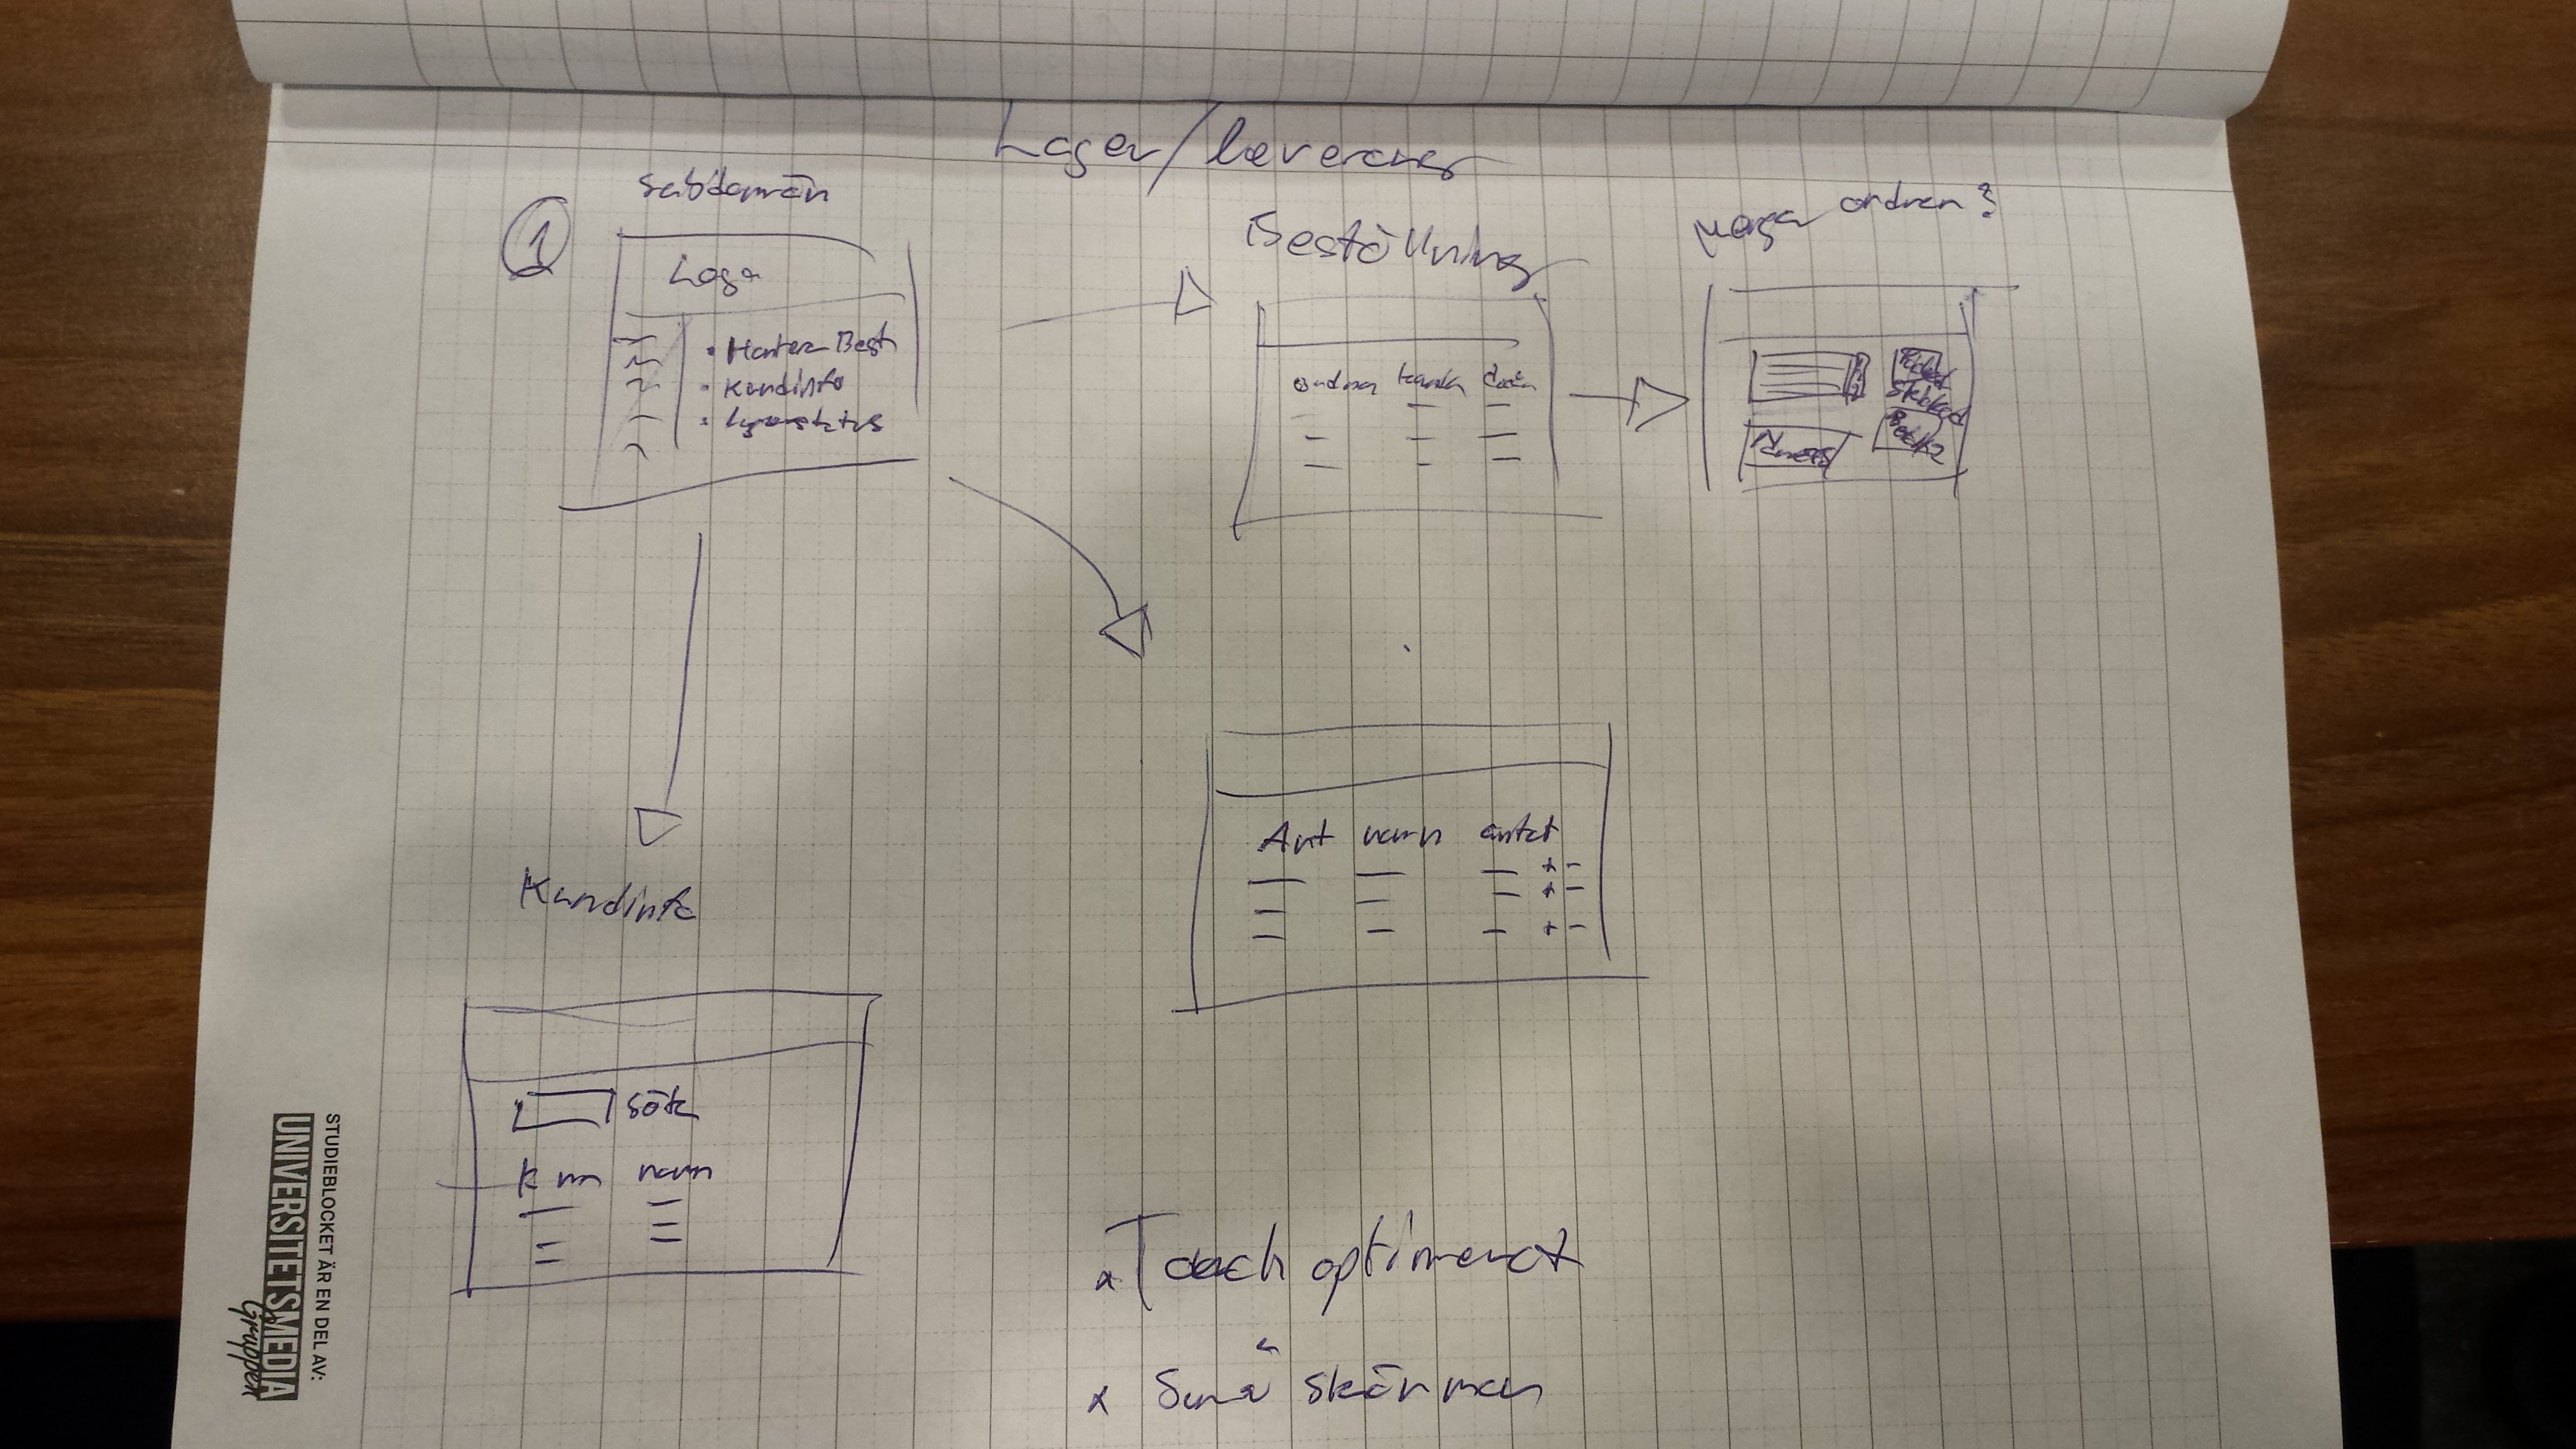
\includegraphics[scale=0.12]{artifacts/Lager.jpeg}
		\caption{}
		\label{fig:2}
	\end{figure}

	\begin{figure}
		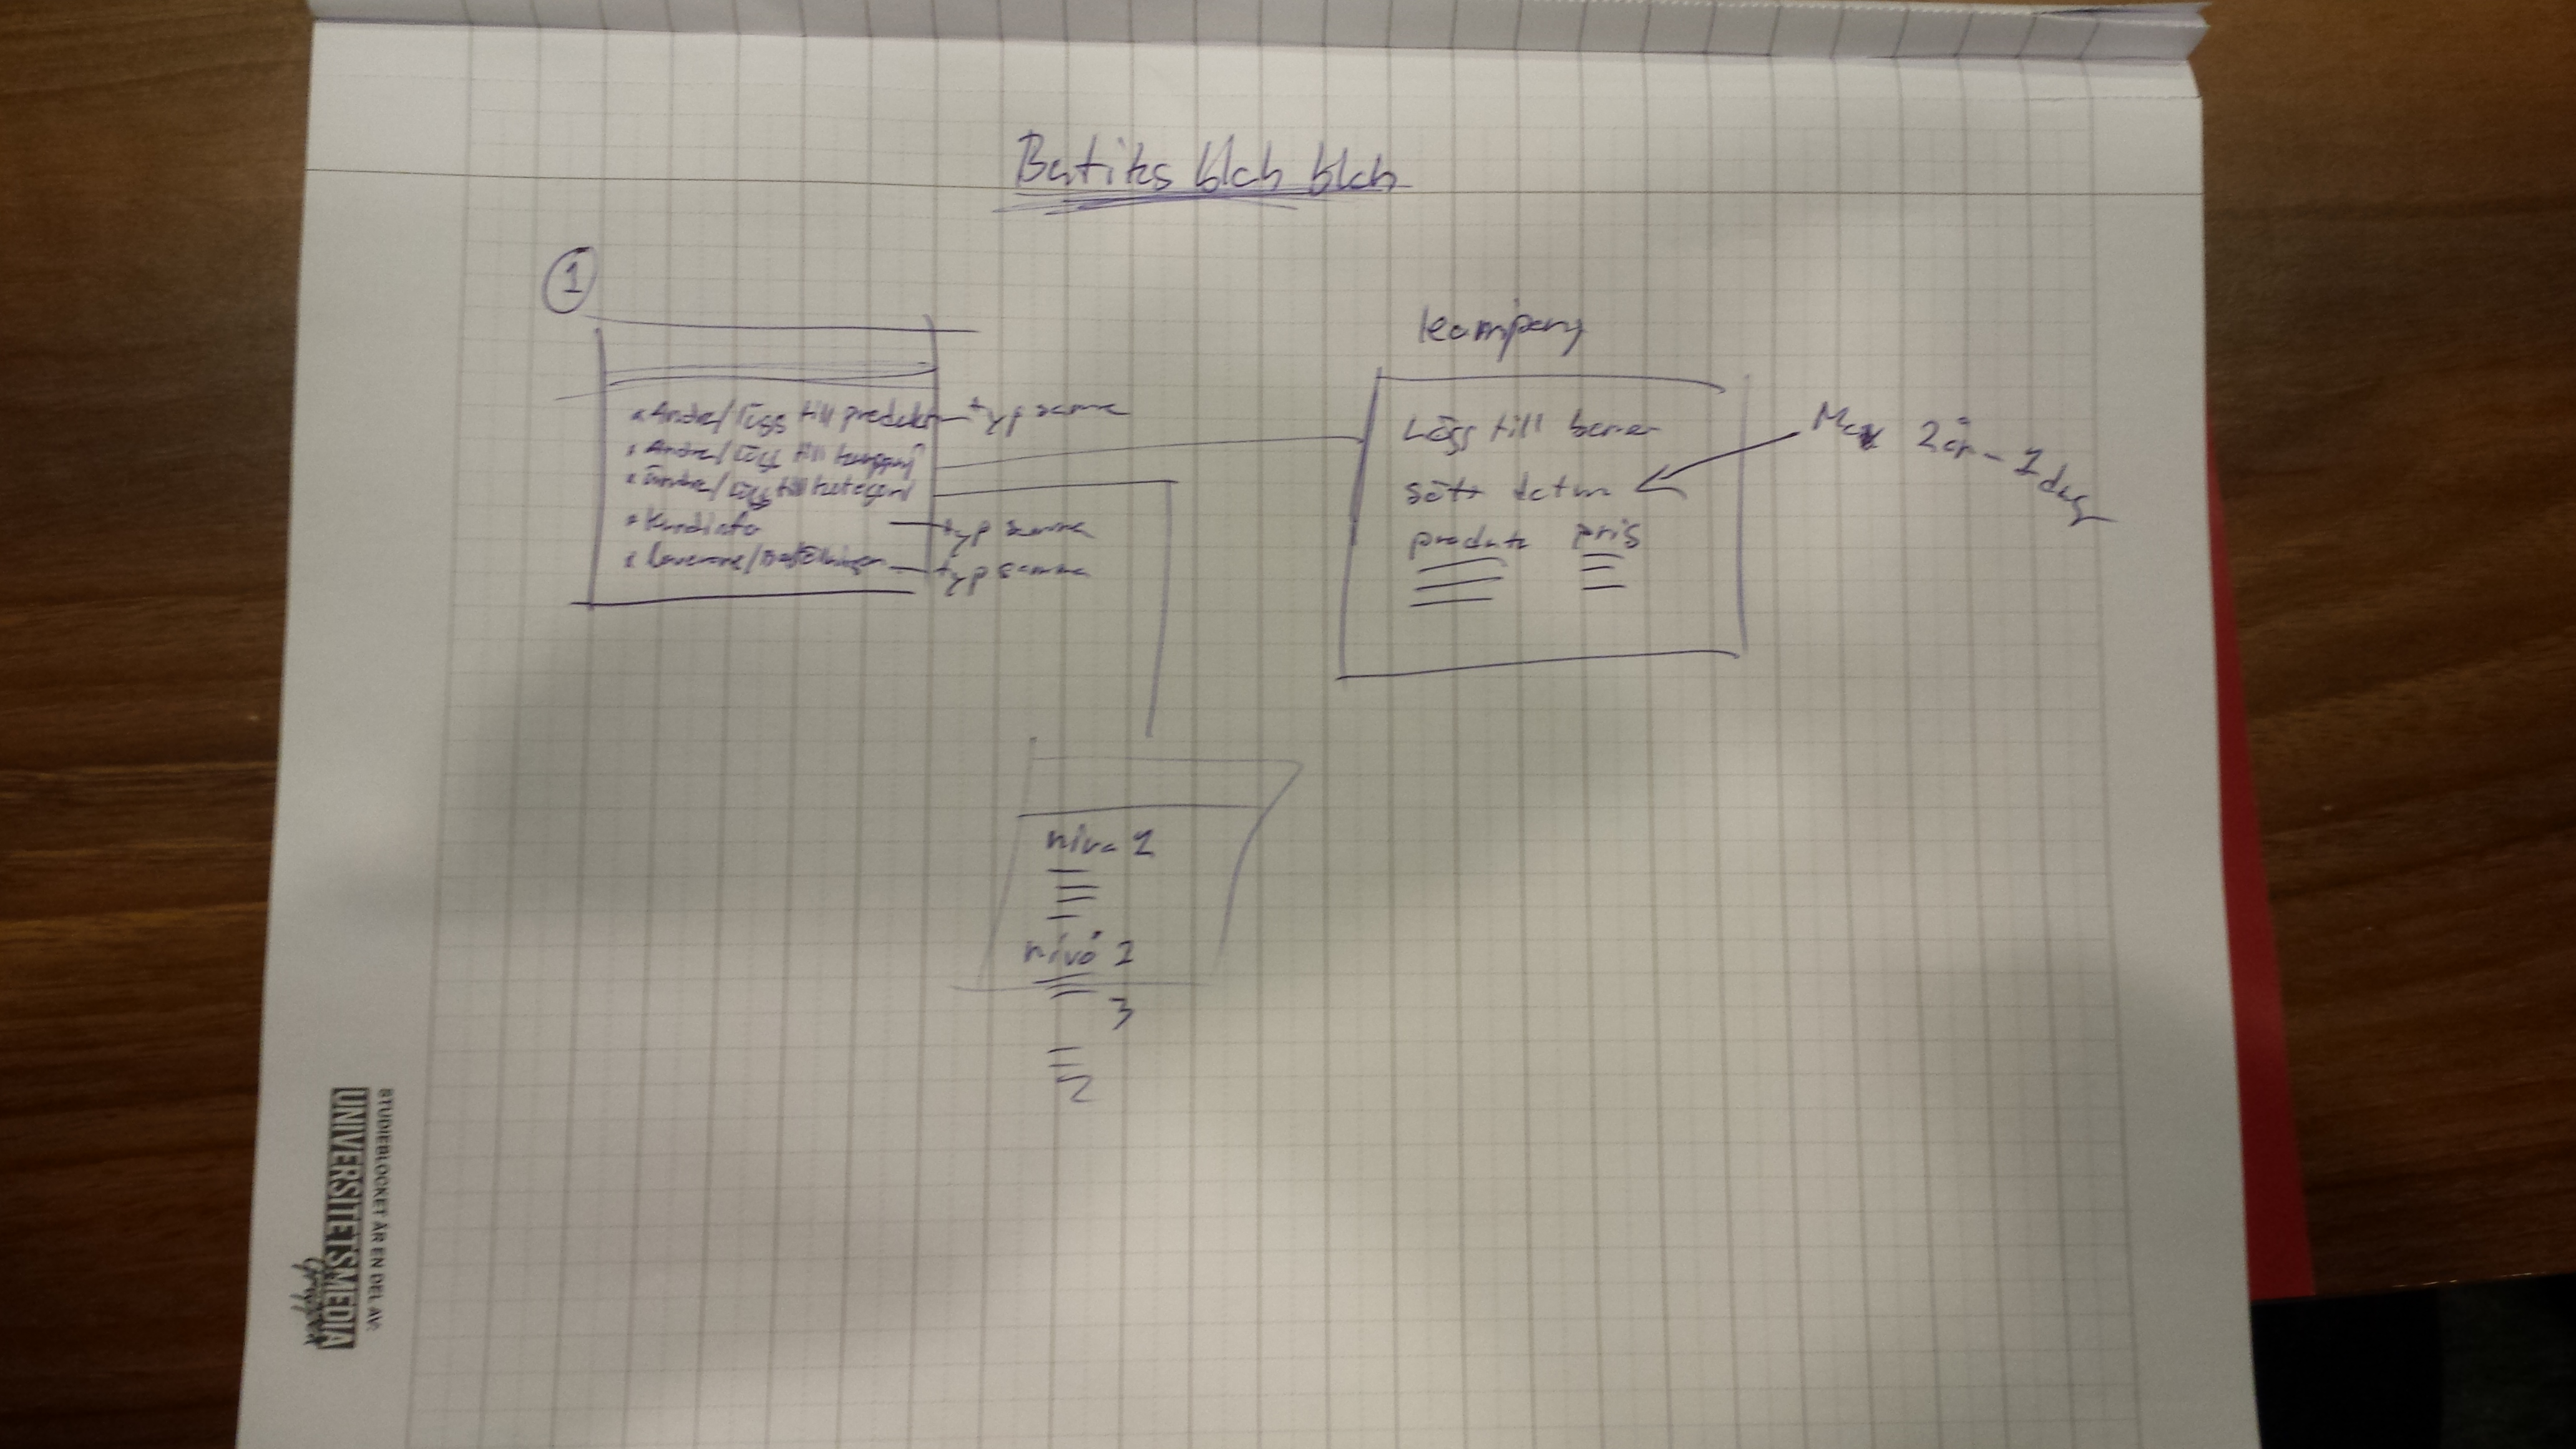
\includegraphics[scale=0.12]{artifacts/ButiksAdmin.jpeg}
		\caption{}
		\label{fig:3}
	\end{figure}

	\begin{figure}
		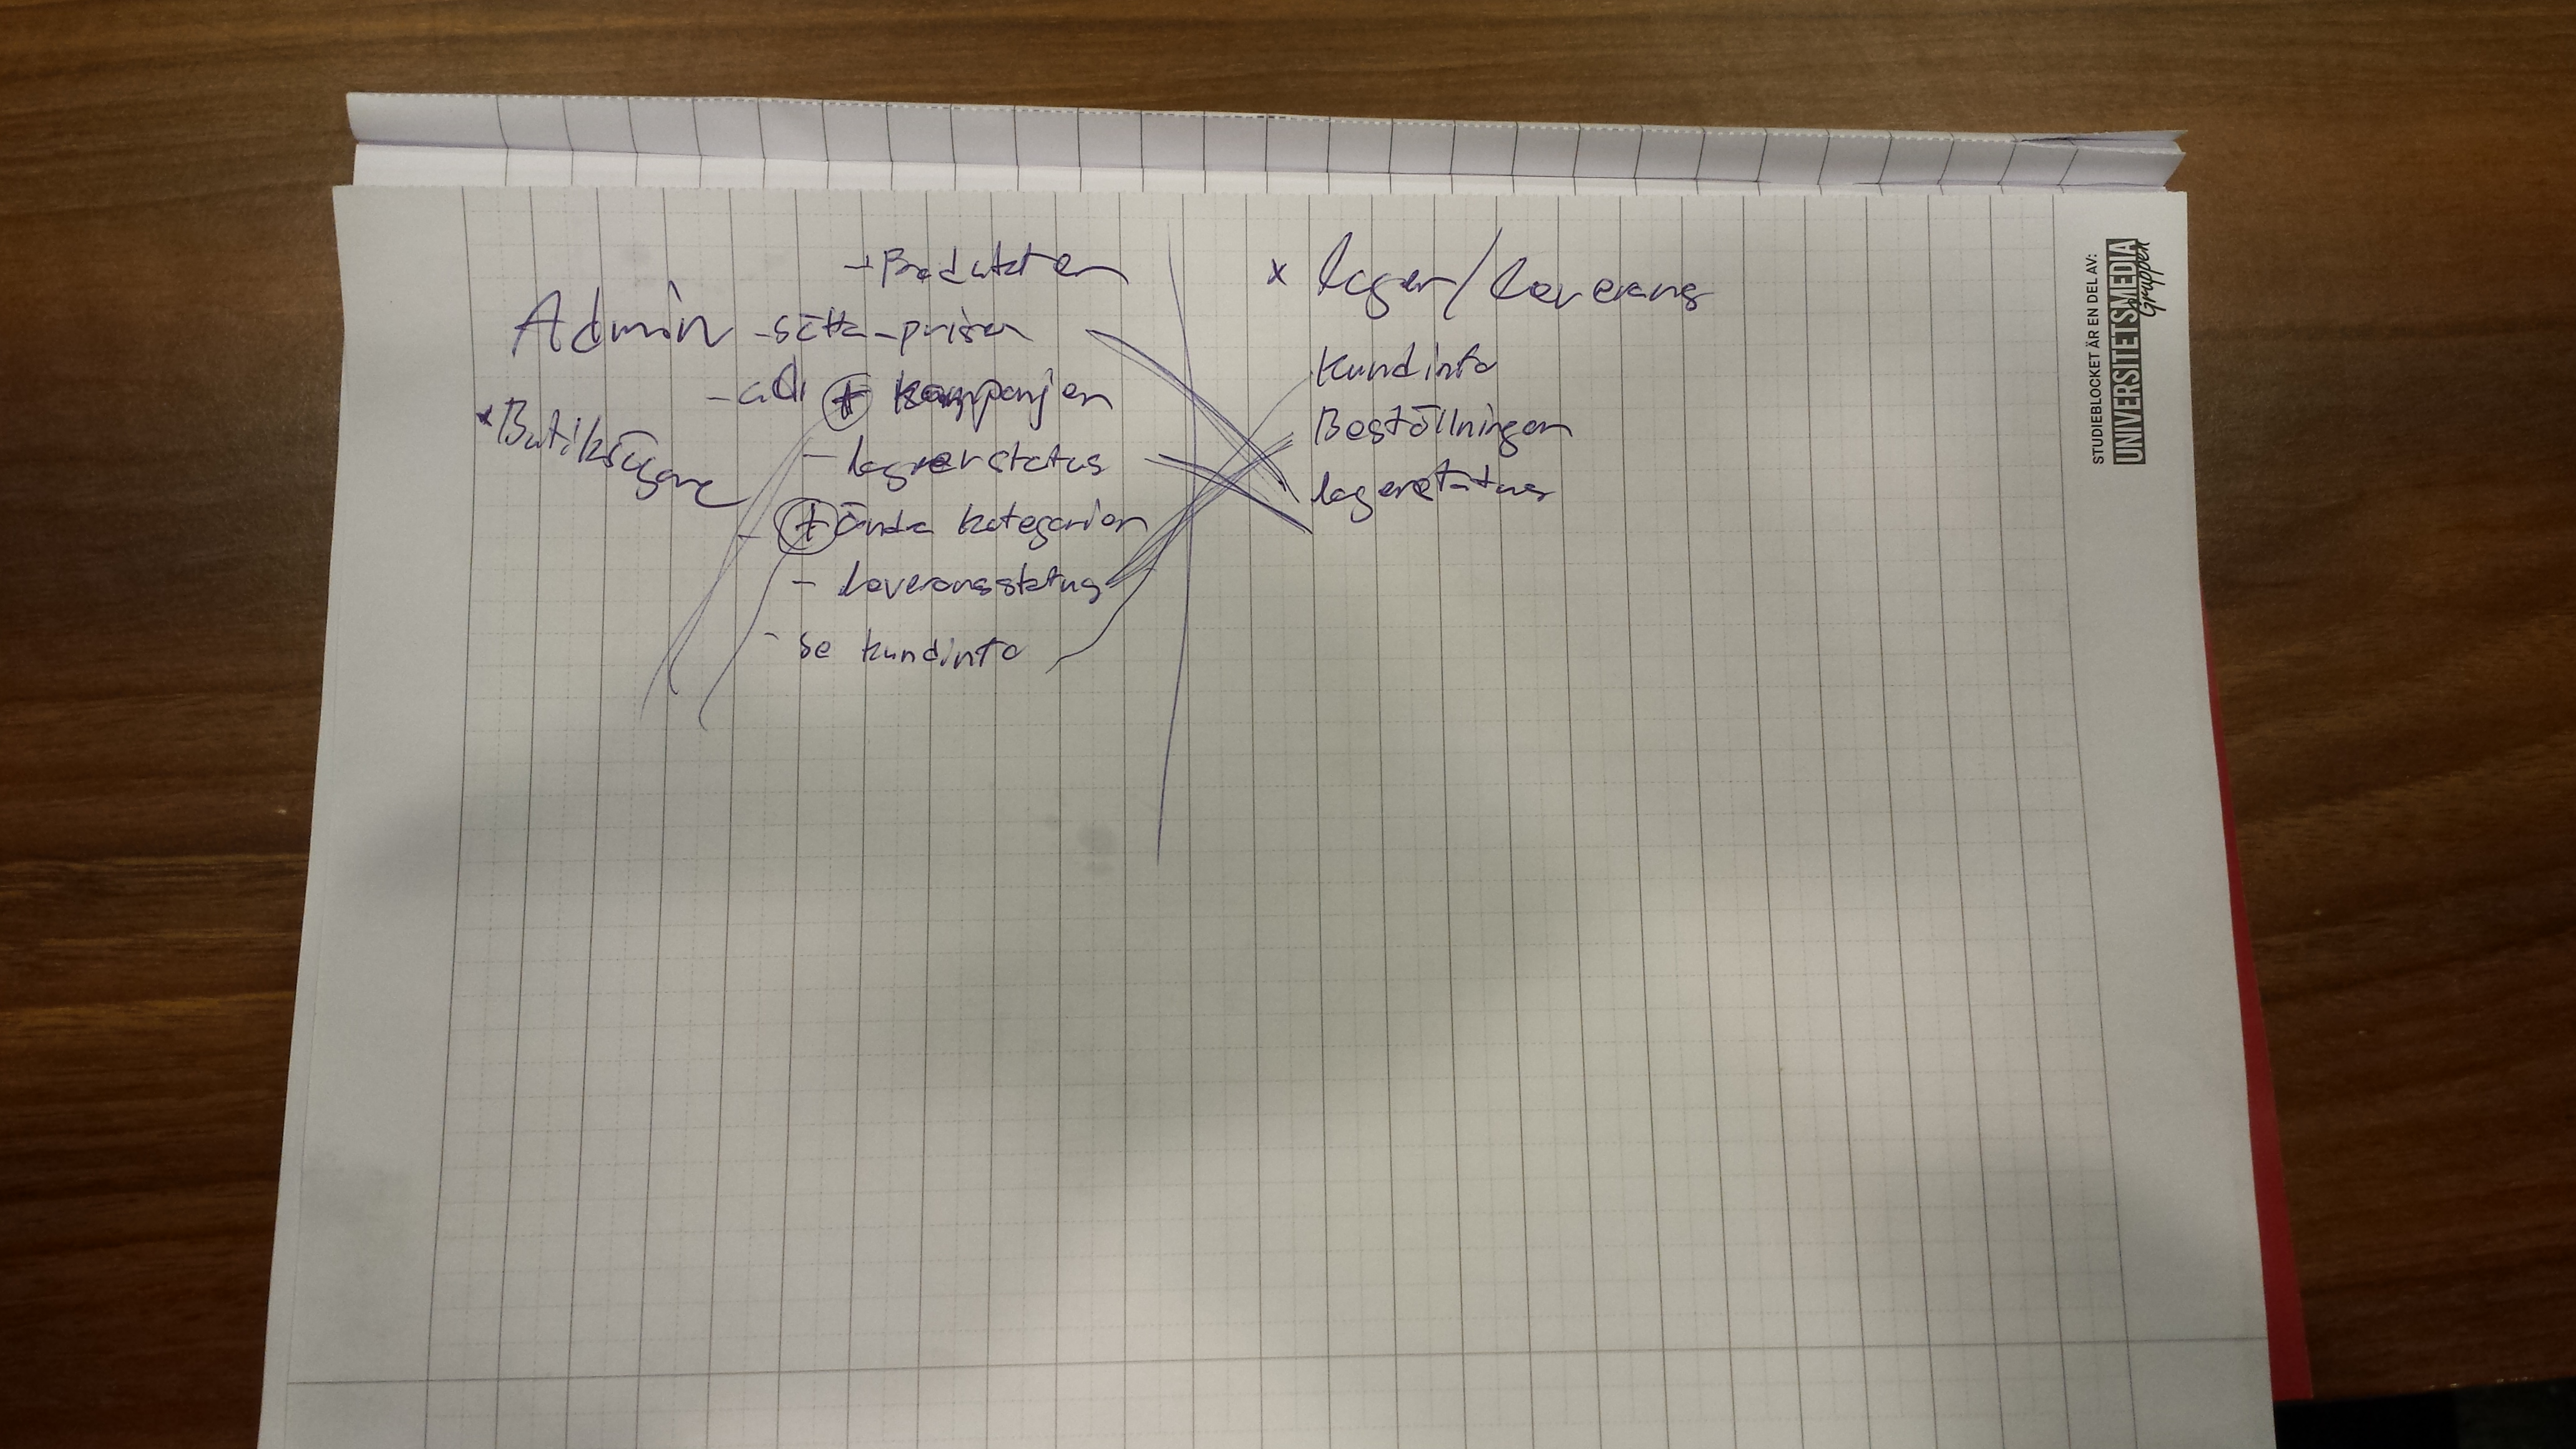
\includegraphics[scale=0.12]{artifacts/Admin.jpeg}
		\caption{}
		\label{fig:4}
	\end{figure}

\section*{System architecture}
\addcontentsline{toc}{section}{System architecture}
	During development we run the system on Ruby on Rails' (RoR) built in web server
	Puma and SQLight3 for simplicity, but intend to move to a MariaDB database
	and a Nginx web server with Phusion Passenger for RoR. We host
	the servers ourselves because it seemed seemed fun, educational and fairly simple.

\section*{Backlog}
\addcontentsline{toc}{section}{backlog}

	The backlog was made after diskussions after breaking down the user stories
	into backlog stories, which were further broken down into tasks. They were
	then given priorities and time estimates. We tried to have a sit down halfway
	through every sprint to see if any stories needed to be broken down into
	smaller stories or if some stories needed to be combined. After that the
	stories would be repriortized and re-estimated.

	\nobrakespace{
		These backlog items were dealt with during this (last) sprint.
		Figure \ref{trello_final} includes a snapshot of the scrum board
		at the end of this sprint. \\
	\begin{tabular}{|l|l|l|l|}
	\addcontentsline{lot}{Backlog}{Spint 4}
		\hline
		\#  & Sprint 4                      & Priority & Time est. \\ \hline
		301 & Startsida                     & 100      & 2         \\ \hline
		302 & Dynamisk meny från kategorier & 90       & 2         \\ \hline
		304 & Produktsida                   & 110      & 4         \\ \hline
		305 & Kundkorg                      & 80       & 8         \\ \hline
		307 & Profilsida (kundkort)         & 45       & 2         \\ \hline
		308 & Orderhistorik                 & 45       & 1         \\ \hline
		309 & Kundinlogg                    & 50       & 2         \\ \hline
		310 & Registrering                  & 60       & 4         \\ \hline
		312 & kommentarer/betygsättning     & 70       & 8         \\ \hline
		313 & Produktkategorier             & 75       & 2         \\ \hline
		400 & Backendinloggning             & 25       & 2         \\ \hline
		1   & Personnummer -/+ hantering    & 5        & 1         \\ \hline
	\end{tabular}
	} \\


	\nobrakespace{
		These stories were put on hold and eventually scrapped from the project. \\
	\begin{tabular}{|l|l|l|l|}
	\addcontentsline{lot}{Backlog}{Left in backlog}
		\hline
		\#  & Left in backlog  & Priority & Time est. \\ \hline
		410 & Kampanjhantering & 10       & 3         \\ \hline
		311 & Produktsökning   & 45       & 1         \\ \hline
		306 & Betalsida        & 5        & 12        \\ \hline
	\end{tabular}
	} \\

	Planing is done at Trello.com
	\url{https://trello.com/b/JxDCHBcm} \\
	This is just a small section of the backlog. For history of all sprints and deeper
	explanation of the backlog items, refer to Trello.

	
	\begin{figure}[h]
		\includegraphics[width=\textwidth]{artifacts/trello_sprint1.png}
		\caption{Screenshot of the scrum board going into the second sprint.}
		\label{fig:trello_sprint1}
	\end{figure}

	\begin{figure}[h]
		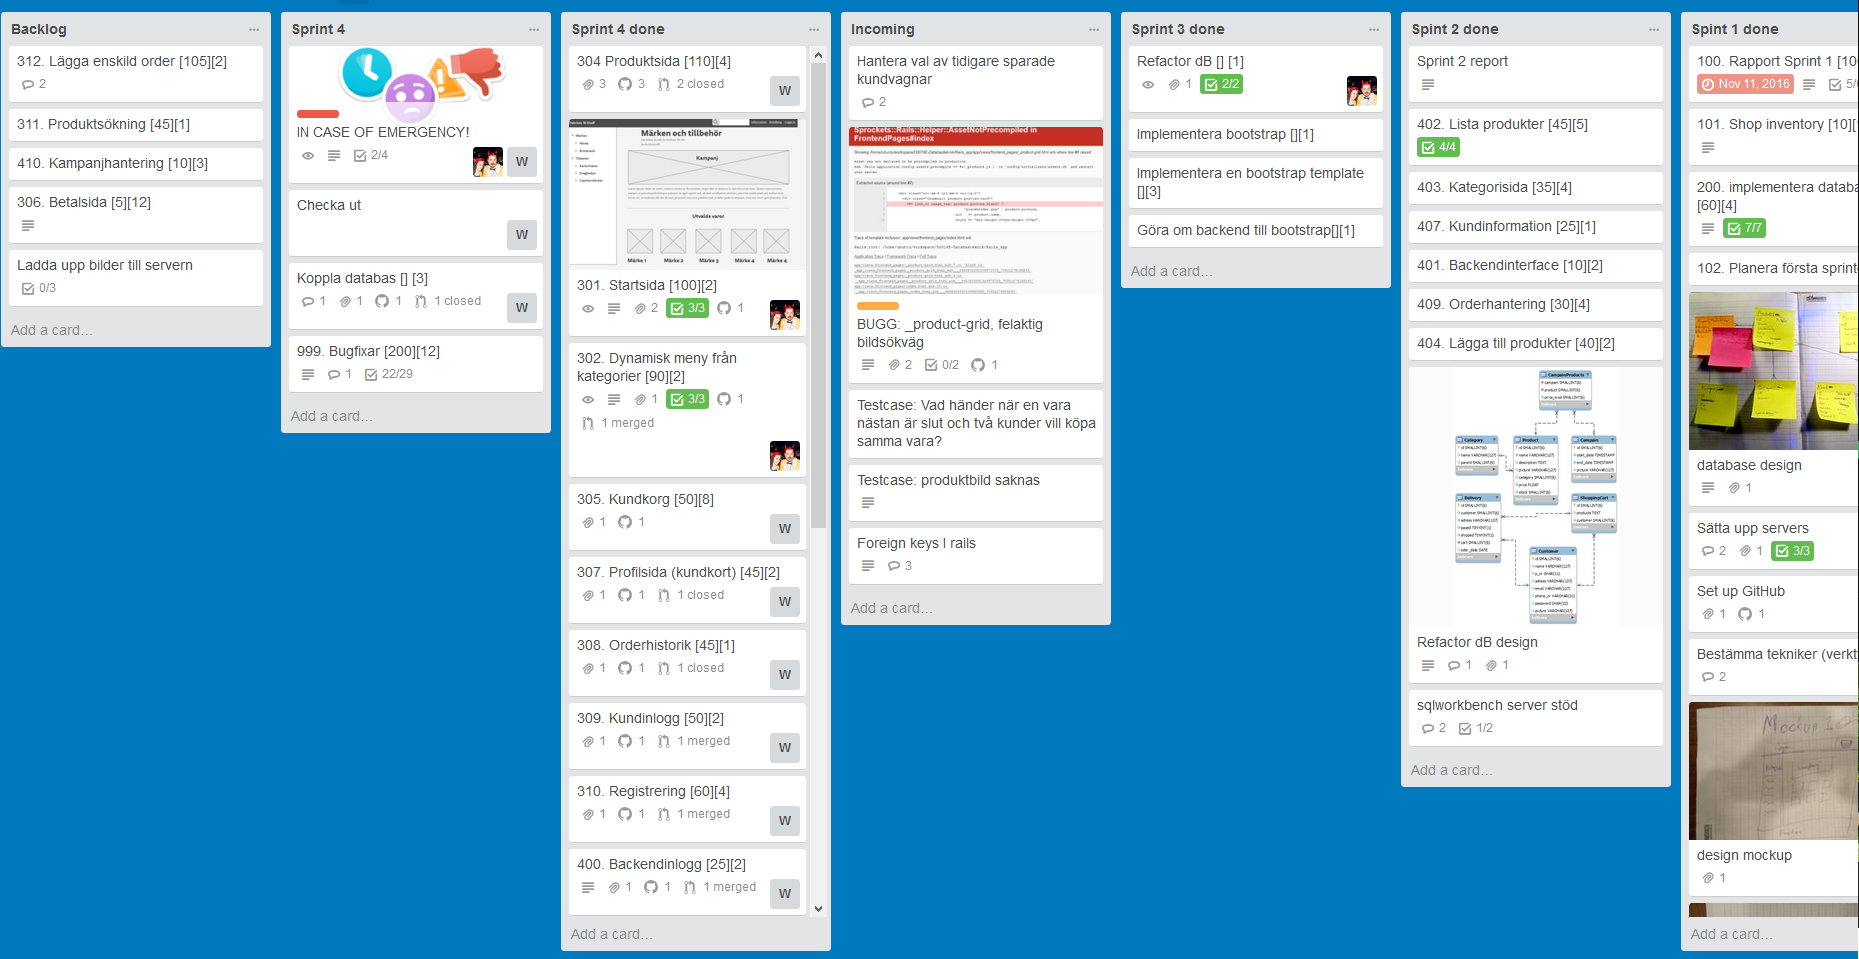
\includegraphics[width=\textwidth]{artifacts/trello_final.png}
		\caption{Screenshot of the current state of the scrum board.}
		\label{fig:trello_final}
	\end{figure}

\section*{Database schema}
\addcontentsline{toc}{section}{Database schema}
See Figure \ref{fig:db}

\begin{figure}
	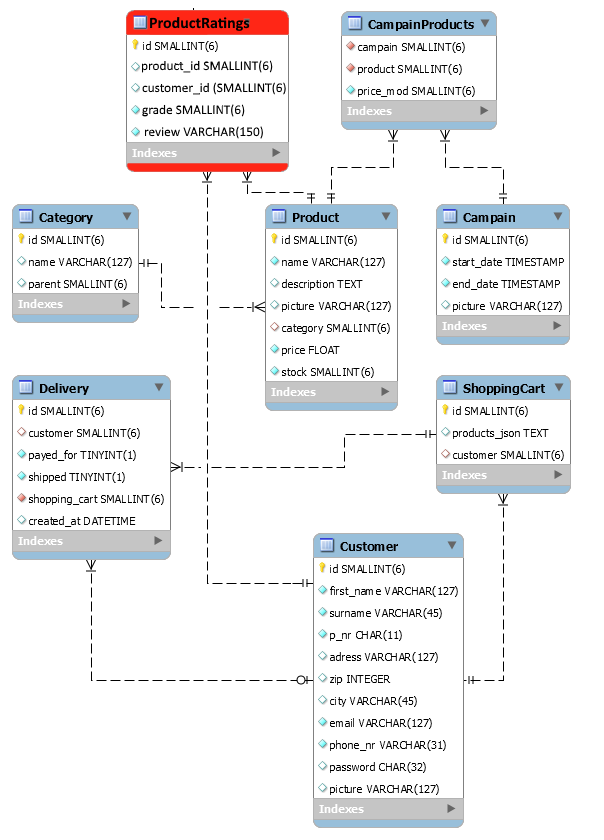
\includegraphics[width=\textwidth]{artifacts/db_implemented_1_3.png}
	\caption{Database design.}
	\label{fig:db}
\end{figure}

\section*{Code}
\addcontentsline{toc}{section}{Code}
All code is available at github.
\url{https://github.com/nikalas/D0018E-Databasteknik.git}

\section*{Test case specifications}
\addcontentsline{toc}{section}{Test case specifications}

% TODO? Did we define more test cases?
% TODO: Should include some unit tests.

	Problem: Item out of stock? \\
		A customer adds a product to the basket. If the product goes out of
		stock before checkout, how is this handled?

	Solution: \\
		At checkout a check is made if the product is still in stock. If not
		the customer is brought back to the 'carts' page and asked to remove
		the product that is no longer available and that the cart has to be
		updated.

\section*{Limitations and improvements}
\addcontentsline{toc}{section}{Limitations and improvements}

	We decided to put off saving payment methods and/or information. Might
	end up re-adding it to the backlog if it looks like we will have time
	to spare. Non-registered customers have also pretty much been put on hold for now.
	Products search, sorting, sale campaigns, and uploading pictures
	through the backend has also been put on hold, since we didn't have
	time to fully implement them.

%TODO: Insert screen shots of whatever Miguel wanted us to add.

\end{document}
